\documentclass[final,3p,times]{elsarticle}

%% Packages required by Computational Materials Science / Elsevier
\usepackage{hyperref}
\usepackage{amsmath,amssymb,amsfonts,bm}
\usepackage{graphicx}
\usepackage{booktabs}
\usepackage{multirow}
\usepackage{array}
\usepackage{microtype}
\usepackage{xcolor}
\usepackage{caption}
\usepackage{subcaption}
\usepackage{url}

\journal{Computational Materials Science}

%% Hyperref configuration
\hypersetup{
    colorlinks=true,
    linkcolor=blue!75!black,
    citecolor=blue!75!black,
    urlcolor=blue!75!black
}

\begin{document}

\begin{frontmatter}

\title{Reproducible Crystal-Graph Learning for Refractive-Index Prediction and Chemical-System-Disjoint Evaluation in Inorganic Materials}

\author{Daksh Kaila\corref{cor1}}
\ead{dkaila_be25@thapar.edu}

\cortext[cor1]{Corresponding author. Department of Computer Science and Engineering, Thapar Institute of Engineering and Technology, Patiala, Punjab 147004, India.}

\affiliation{organization={Department of Computer Science and Engineering, Thapar Institute of Engineering and Technology},
            city={Patiala},
            state={Punjab},
            postcode={147004},
            country={India}}

\begin{abstract}
Accelerated discovery of optical and dielectric crystals relies on accurate data-driven surrogates for the refractive index $n$, yet benchmark metrics frequently suffer from inadvertent test-set monitoring and fail to reflect generalization across distinct chemical spaces. Here, we systematically audit classical descriptor pipelines and periodic graph architectures on the $N = 4{,}764$ MatBench dielectric benchmark. Enforcing strict nested validation with fold-local scaling, an RBF-SVR baseline achieves an MAE of $0.3124 \pm 0.0812$, outperforming our in-house implementation of the canonical CGCNN architecture ($0.3298 \pm 0.0800$), while demonstrating that inadvertent test-monitored checkpoint selection during exploratory training can artificially deflate baseline error estimates (e.g., to $0.2068$ on an individual fold). We then present DualHead--LogDirect GNN, an architecture coupling tabulated elemental ground-state priors, three-body Chebyshev angular projections, a 12-dimensional macroscopic packing vector, and dual bounded readout heads. On official MatBench folds, it reaches a development-stage MAE of $0.2909 \pm 0.0860$ and median absolute error of $0.0631 \pm 0.0023$. When retrained from scratch under chemical-system-disjoint five-fold cross-validation across 3,169 non-overlapping chemical systems, the frozen model retains robust rank ordering ($\rho = 0.9331$) and an MAE of $0.2973 \pm 0.0237$, representing a 2.2\% higher MAE than the official-fold development-stage estimate. Residual diagnostics show that exceptional accuracy across typical insulators ($n \le 3.0$, $\text{MedAE} = 0.0510$) coexists with severe heteroskedastic underprediction in the sparse high-index tail ($n > 8.0$). This work provides a rigorous materials-informatics framework distinguishing exploratory benchmark tuning from frozen chemical-system-disjoint evaluation.
\end{abstract}

\begin{keyword}
Crystal Graph Neural Networks \sep Refractive Index \sep Materials Informatics \sep Chemical-System-Disjoint Evaluation \sep Benchmark Reproducibility \sep MatBench
\end{keyword}

\end{frontmatter}

\section{Introduction}
The optical refractive index $n$ governs electromagnetic propagation in condensed matter and dictates phase velocity, dispersion, and dielectric polarization. Accurate estimation of $n$ is central to screening optical coatings, high-power dielectric mirrors, photonic waveguides, and metasurfaces \cite{petousis2017high, ramprasad2017machine, dunn2020benchmarking}. Although density functional perturbation theory (DFPT) computes high-frequency dielectric tensors from first principles, reciprocal-space convergence and electronic response calculations incur steep computational costs that restrict exhaustive exploratory searches across large crystalline repositories \cite{petousis2017high}. Consequently, supervised machine learning (ML) models trained on curated electronic structure databases have gained traction as fast surrogate filters \cite{ward2016general, xie2018crystal, chen2019graph}.

Standardized benchmarks, in particular the MatBench suite \cite{dunn2020benchmarking}, have accelerated progress by providing uniform cross-validation folds. For the \texttt{matbench\_dielectric} task ($N = 4{,}764$), reported models span automated feature-selection frameworks such as MODNet \cite{de2021robust} and periodic crystal graph neural networks (GNNs) including CGCNN \cite{xie2018crystal}, MEGNet \cite{chen2019graph}, SchNet \cite{schutt2017schnet}, and ALIGNN \cite{choudhary2021atomistic}. However, benchmarking practices in materials informatics face three recurring methodological pitfalls.

First, deep learning architectures in materials science risk subtle data leakage when early stopping, checkpoint selection, or learning rate schedules are guided by outer-test loss trajectories \cite{artrith2021best}. Such inadvertent test monitoring produces optimistically biased metrics that fail to replicate on genuine out-of-sample data. Second, repeated architecture tuning on fixed benchmark splits encourages post hoc selection and leaderboard overclaiming, where incremental empirical gains on validation folds are asserted as definitive superiority despite wide differences in compute budgets, feature representations, and optimization protocols. Third, standard cross-validation randomly distributes compositions across partitions. In prospective materials screening, discovery algorithms target chemical spaces whose exact elemental combinations are absent from training databases \cite{xiong2023evaluating}, exposing models to distribution shifts that standard random splits cannot detect.

To address these issues, this study presents a rigorous reproducibility audit and an inductive crystal-graph architecture for refractive-index prediction. First, auditing classical and graph baselines under strict nested validation reveals that an RBF-SVR pipeline ($0.3124 \pm 0.0812$ MAE) outperforms our independently trained implementation of the canonical CGCNN architecture ($0.3298 \pm 0.0800$ MAE), while highlighting how preliminary test-monitored checkpoint selection can produce artificially optimistic error estimates that fail to hold under strict leak-free protocols. Second, we introduce DualHead--LogDirect GNN, which integrates elemental ground-state priors, three-body angular features, a 12-dimensional macroscopic packing vector, and dual bounded readout heads, reaching a development-stage five-fold MAE of $0.2909 \pm 0.0860$ and median absolute error of $0.0631 \pm 0.0023$. Third, retraining the frozen model from scratch under chemical-system-disjoint 5-fold cross-validation across 3,169 non-overlapping chemical systems establishes that the architecture yields an MAE of $0.2973 \pm 0.0237$ (a 2.2\% higher MAE than the official-fold development-stage estimate) and retains a rank correlation of $\rho = 0.9331$. Finally, detailed residual diagnostics demonstrate that while the model achieves high precision across typical optical insulators ($n \le 3.0$), severe heteroskedasticity and systematic underprediction emerge in the extreme tail ($n > 8.0$), clarifying the practical reliability boundaries of crystal-graph screening.

\section{Materials and Methods}

\subsection{Benchmark Dataset and Target Characteristics}
We evaluate all models on the official MatBench v0.1 \texttt{matbench\_dielectric} benchmark \cite{dunn2020benchmarking}. The dataset comprises $N = 4{,}764$ inorganic crystalline structures computed with density functional perturbation theory within the Materials Project \cite{jain2013commentary, petousis2017high}.

The target is the unitless scalar refractive-index value supplied by the MatBench dielectric task and derived from Materials Project dielectric calculations \cite{dunn2020benchmarking, petousis2017high}. It is a scalar benchmark representation of optical response; it does not resolve dielectric-tensor anisotropy, principal refractive indices, wavelength-dependent dispersion, or optical absorption. The target distribution is heavily right-skewed: the median refractive index is $2.071$, the mean is $2.428$, 95\% of samples lie below $n = 4.35$, while extreme entries extend up to $n = 62.06$.

\subsection{Fold-Local Evaluation and Checkpoint-Selection Protocol}
To reduce within-run evaluation bias, we used the following fold-local protocol:
\begin{enumerate}
    \item \textbf{Official Outer Five-Fold Partition}: We employ the exact five folds defined by the official MatBench v0.1 API ($N = 4{,}764$, with outer test folds of 953, 953, 953, 953, and 952 materials). Saved fold manifests were hashed for integrity and checked against the MatBench API splits for zero train--test overlap ($T_{f,\mathrm{train}} \cap T_{f,\mathrm{test}} = \emptyset$) and complete test coverage.
    \item \textbf{Inner-Validation Checkpointing}: Outer training sets ($N \approx 3,811$) are partitioned into an 85\% inner-train split and a 15\% inner-validation split using deterministic pseudo-random seeds. Model optimization, learning rate scheduling, and checkpoint selection are monitored exclusively on inner-validation performance.
    \item \textbf{Frozen Single-Pass Outer-Test Evaluation}: Within each finalized run, outer-test labels and metrics were not used for training, checkpoint selection, or hyperparameter selection. Checkpoints selected by inner validation were evaluated once on the unseen outer-test fold.
\end{enumerate}

\subsection{Classical Feature Engineering and Baseline Pipelines}
To establish robust classical benchmarks, crystal structures were featurized into a 153-dimensional descriptor representation using \texttt{matminer} \cite{ward2018matminer}:
\begin{enumerate}
    \item \textit{Stoichiometric elemental attributes (132)}: Derived using the Magpie attribute library \cite{ward2016general}, calculating composition-weighted moments (mean, variance, span, minimum, and maximum) for atomic radii, Pauling electronegativities, valence electron configurations, covalent dimensions, and ground-state elemental properties.
    \item \textit{Crystallographic symmetry features (12)}: Extracted from space-group analyses \cite{ong2013python}, encompassing the space-group integer ($1 \le SG \le 230$), one-hot categorical vectors for the seven crystal systems, and Bravais lattice classifications.
    \item \textit{Electrostatic spectrum (9)}: Calculated from the periodic sine-Coulomb matrix \cite{ong2013python}, retaining the 9 largest eigenvalues to encode electrostatic interactions and core nuclear charge distributions under periodic unit-cell boundary conditions.
\end{enumerate}
All preprocessing transformations, including median missing-value imputation and feature standardization scalers, were fit strictly inside each inner-training fold to maintain fold-local preprocessing. Classical models evaluated include Ridge regression, Linear Support Vector Regression (SVR), Polynomial SVR ($d=3$), Radial Basis Function SVR (RBF-SVR), and Random Forest \cite{pedregosa2011scikit}.

\subsection{Primary Crystal Graph Architecture: DualHead--LogDirect GNN}
To capture periodic crystal geometry directly, we construct crystal graphs as a periodic atomistic graph. For the primary DualHead--LogDirect GNN architecture (implemented as \texttt{DualHead\_LogDirect\_GNN}), graphs were constructed using a radial cutoff of $R_{\mathrm{cut}} = 6.0$~\AA, truncated to the 12 nearest neighbors within the $R_{\mathrm{cut}} = 6.0$~\AA\ cutoff sphere. Interatomic distances $r_{ij}$ were expanded using 41 Gaussian radial basis functions (RBF):
\begin{equation}
    e_{ij, k} = \exp\left(-\gamma (r_{ij} - \mu_k)^2\right), \quad k \in \{1, \dots, 41\},
\end{equation}
where $\mu_k$ are uniformly spaced centers from $0.0$ to $6.0$~\AA\ with step $\Delta\mu = 0.15$~\AA, and the Gaussian width parameter is $\gamma = 1/\sigma^2 \approx 44.44$~\AA$^{-2}$ ($\sigma = 0.15$~\AA). Distance expansions were complemented by an inverse distance channel $1/(r_{ij} + 0.01)$ and 16 Chebyshev polynomial features of the local bond-angle cosine $\cos\theta_{jik}$, averaged over all eligible neighbor triplets associated with each directed edge, yielding a 58-dimensional edge attribute vector $\mathbf{e}_{ij}$. For a directed edge $(i, j)$, $i$ is the angle vertex and the local angle features are obtained from all triplets $(j, i, k)$, $k \in \mathcal{N}(i) \setminus \{j\}$; with unit displacements $\hat{\mathbf{r}}_{ij}$ and $\hat{\mathbf{r}}_{ik}$, the bond-angle cosine is $\cos\theta_{jik} = \hat{\mathbf{r}}_{ij} \cdot \hat{\mathbf{r}}_{ik}$, which is expanded into 16 Chebyshev polynomial features and averaged over all eligible neighbor triplets. Baseline CGCNN variants used their separately documented edge expansions (48 Gaussian RBFs at an $8.0$~\AA\ cutoff without angular basis features; Supplementary Table S3).

The DualHead--LogDirect GNN architecture incorporates three domain-specific inductive biases:
\begin{enumerate}
    \item \textbf{Atomic Embeddings and Eight Tabulated Elemental Descriptors}: Atom nodes receive learnable embeddings from atomic number $Z \in \{1, \dots, 100\}$ (48 dimensions) concatenated with an 8-dimensional normalized elemental descriptor prior vector extracted from \texttt{pymatgen.core.Element} \cite{ong2013python}: Pauling electronegativity ($X$), atomic radius ($r$), atomic mass ($m$), periodic table group ($g$), periodic table row ($\text{row}$), first ionization energy ($\text{IE}$), molar volume ($V_{\mathrm{mol}}$), and maximum oxidation state ($\text{ox}_{\max}$). These represent tabulated elemental ground-state quantities rather than physically realized in-crystal valence or polarizability states. All eight tabulated elemental descriptors are normalized using z-score standardization across $Z \in [1, 100]$ (Supplementary Note 1, Table S1). Polarizability and valence electron counts are not included in the GNN node feature vector.
    \item \textbf{Hierarchical Convolutions, Global State Vector, and Message Aggregation}: The network employs 3 hierarchical interaction layers. In each layer, edge attributes $\mathbf{e}_{ij}$, atom node representations $\mathbf{h}_i$, and a 12-dimensional global structural--compositional descriptor vector $\mathbf{u}$ are updated via multi-layer perceptron (MLP) blocks equipped with LayerNorm and SiLU activations. Edge representations are updated as:
    \begin{equation}
        \mathbf{e}_{ij}^{(l+1)} = \mathbf{e}_{ij}^{(l)} + \mathrm{MLP}_{\mathbf{e}}\left([\mathbf{h}_i^{(l)} \parallel \mathbf{h}_j^{(l)} \parallel \mathbf{e}_{ij}^{(l)} \parallel \mathbf{u}_{\mathrm{edge}}^{(l)}]\right).
    \end{equation}
    Messages were summed over retained neighbors without degree normalization:
    \begin{equation}
        \mathbf{m}_i^{(l+1)} = \sum_{j \in \mathcal{N}(i)} \mathbf{e}_{ij}^{(l+1)}.
    \end{equation}
    Atom node representations are subsequently updated with residual connection:
    \begin{equation}
        \mathbf{h}_i^{(l+1)} = \mathbf{h}_i^{(l)} + \mathrm{MLP}_{\mathbf{v}}\left([\mathbf{h}_i^{(l)} \parallel \mathbf{m}_i^{(l+1)} \parallel \mathbf{u}_{\mathrm{node}}^{(l)}]\right),
    \end{equation}
    where LayerNorm is applied inside the MLP blocks before residual addition. The 12-dimensional global structural--compositional descriptor vector $\mathbf{u}$ combines density, cell geometry, packing, composition-derived elemental statistics, graph coordination, and lattice aspect ratio: (1) mass density $\rho$, (2) volume per atom $V/N$, (3) atomic packing fraction $\phi$, (4) element count $N_{\mathrm{elem}}$, (5) stoichiometric mean Pauling electronegativity $\bar{X}$, (6) electronegativity range $\Delta X$, (7) mean atomic radius $\bar{r}$, (8) mean periodic group number $\bar{g}$, (9) mean elemental molar volume $\bar{V}_{\mathrm{mol}}$, (10) average graph coordination number $\bar{z}$, (11) an engineered dimensionless packing descriptor $\eta_{\mathrm{pack}} = \phi (V/N)/\bar{r}^3$, and (12) lattice aspect ratio $c/a$. All geometric quantities were expressed in \AA-based units before construction of $\eta_{\mathrm{pack}}$, making the ratio dimensionless; correlations among global descriptors were retained intentionally as model inputs and are documented in Supplementary Note 1. The 12-dimensional global vector is specified in Supplementary Table S2. Its scaler was fit on the inner-training split only and then applied to validation and outer-test structures. For internal benchmarking, \texttt{Global\_CGNN} is an earlier development-stage comparator that conditions 4 gated interaction layers on a 4-variable global vector ($V/N, \rho, \bar{Z}, \bar{z}$) without angular edge features (Supplementary Table S3).
    \item \textbf{Dual Readout Heads and Multitask Objective}: Crystal-level pooling yields a latent vector $\mathbf{h}_{\mathrm{crystal}} = [\frac{1}{N_{\mathrm{atoms}}} \sum_i \mathbf{h}_i \parallel \mathbf{u}]$. To balance optimization pressure from the densely sampled central region and the sparse high-index tail, the network jointly predicts:
    \begin{align}
        \hat{n}_{\mathrm{direct}} &= 1.0 + \operatorname{Softplus}(\mathbf{W}_d \mathbf{h}_{\mathrm{crystal}} + b_d), \\
        \hat{z}_{\mathrm{log}} &= \mathbf{W}_\ell \mathbf{h}_{\mathrm{crystal}} + b_\ell, \quad \text{modeling } z = \ln(n - 0.99).
    \end{align}
    The network is optimized using a joint multitask Smooth L1 loss \cite{huber1964robust} (PyTorch's \texttt{SmoothL1Loss} with transition parameter $\beta = 0.15$):
    \begin{equation}
        \mathcal{L} = \mathcal{L}_{\mathrm{SmoothL1}}(\hat{n}_{\mathrm{direct}}, y; \beta=0.15) + \lambda \mathcal{L}_{\mathrm{SmoothL1}}(\hat{z}_{\mathrm{log}}, \ln(y - 0.99); \beta=0.15),
    \end{equation}
    with $\lambda = 0.5$. The blended inference prediction is:
    \begin{equation}
        \hat{n} = \frac{1}{2}\hat{n}_{\mathrm{direct}} + \frac{1}{2}\left(0.99 + \exp(\hat{z}_{\mathrm{log}})\right).
    \end{equation}
\end{enumerate}

\paragraph{Architectural Inductive Biases Relative to Canonical Crystal GNN Baselines}
To clarify the design rationale compared with canonical crystal graph neural networks considered in this benchmark---such as CGCNN \cite{xie2018crystal}, MEGNet \cite{chen2019graph}, SchNet \cite{schutt2017schnet}, and ALIGNN \cite{choudhary2021atomistic}---we highlight three targeted architectural inductive biases:
\begin{enumerate}
    \item \textbf{Tri-Channel Inductive Prior Featurization}: Whereas baseline crystal GNN formulations such as canonical CGCNN rely strictly on discrete atomic number embeddings and scalar pairwise bond distances, DualHead--LogDirect GNN incorporates domain-specific physical priors across all three graph topological levels simultaneously: (i) atom nodes concatenate learned $Z$-embeddings with eight tabulated elemental physical ground-state properties ($X, r, m, g, \text{row}, \text{IE}, V_{\mathrm{mol}}, \text{ox}_{\max}$); (ii) directed edges combine 41 Gaussian radial basis functions, an inverse-distance electrostatic channel, and 16 Chebyshev polynomial projections of local bond angles $\cos\theta_{jik}$ averaged over neighbor triplets, capturing 3-body angular geometry without the memory overhead of explicit line graphs; and (iii) a 12-dimensional macroscopic structural--compositional vector captures packing, density, coordination, and unit-cell aspect ratio.
    \item \textbf{Hierarchical 3-Way Message Passing}: In contrast to basic crystal convolutions where message passing is confined to local atom--atom or atom--bond updates, our architecture implements bidirectional, three-way interaction layers. Edge representations are updated conditioned on incident node states and global state $\mathbf{u}$; node representations are updated conditioned on aggregated edge messages and global state $\mathbf{u}$; and crystal-level pooling explicitly retains $\mathbf{u}$. This enables macroscopic unit-cell constraints (e.g., density and packing fraction) to modulate microscopic message propagation directly.
    \item \textbf{Dual Bounded-Output Readout with Joint Direct--Log Multitask Loss}: In the canonical crystal-GNN baselines considered in this study, property prediction uses a conventional single regression head optimized with standard loss functions. For optical refractive index, this conventional design can suffer from two specific challenges: generating unphysical sub-unity predictions ($n < 1.0$), and encountering numerical optimization difficulties from the heavy right-skewed target distribution ($n$ up to $62.06$). DualHead--LogDirect GNN couples a direct readout head equipped with a Softplus barrier ($\hat{n}_{\mathrm{direct}} = 1.0 + \operatorname{Softplus}(z_d)$, enforcing the physical constraint $\hat{n}_{\mathrm{direct}} \ge 1.0$) with a logarithmic readout head ($\hat{z}_{\mathrm{log}} = \mathbf{W}_\ell \mathbf{h}_{\mathrm{crystal}} + b_\ell$, modeling $\ln(n - 0.99)$ under smooth L1 loss \cite{huber1964robust}). This formulation simultaneously enforces physical lower-bound integrity, compresses the dynamic range of high-index outliers, and balances gradient backpropagation between typical crystals and extreme optical materials.
\end{enumerate}

\subsection{Chemical-System-Disjoint Grouped Evaluation Protocol}
The standard MatBench folds are not explicitly constrained to prevent related chemical systems from appearing across train and test partitions. To test robustness when exact chemical systems are absent from the training partition, we partitioned the 4,764 materials into 3,169 unique elemental chemical systems (defined by the sorted set of constituent chemical elements). We enforce a five-fold \texttt{GroupKFold} cross-validation partition using scikit-learn (version 1.9.0, deterministic ordering with \texttt{shuffle=False}) grouped strictly by chemical system:
\begin{equation}
    \mathcal{S}(T_{f,\mathrm{train}}) \cap \mathcal{S}(T_{f,\mathrm{test}}) = \emptyset \quad \forall f \in \{0, 1, 2, 3, 4\},
\end{equation}
where $\mathcal{S}(\cdot)$ maps a material subset to its constituent chemical systems. All group assignments and fold manifests were pre-saved and verified for zero chemical-system overlap prior to training. Within each grouped outer training set, the inner validation split (15\%) was partitioned pseudo-randomly for epoch and checkpoint selection; the inner validation split was used only for checkpoint selection and was not chemical-system-grouped; the chemical-system constraint applies to the outer grouped evaluation.

\begin{quote}
\small
\textit{Methodological Caveat}: The grouped split prevents an identical chemical system from occurring in both train and test. It provides a grouped extrapolation stress test rather than standard random cross-validation, but does not guarantee complete extrapolation beyond related compositions, shared elements, or crystal prototypes.
\end{quote}

\subsection{Computational Implementation and Reproducibility}
All neural network models were implemented in PyTorch \texttt{2.14.0+cu126} \cite{paszke2019pytorch}. The DualHead--LogDirect GNN architecture comprises 150,578 trainable parameters. Models were optimized using AdamW \cite{kingma2014adam, loshchilov2017decoupled} with an initial learning rate of $1.8 \times 10^{-3}$, weight decay of $1 \times 10^{-4}$, batch size of 64, and CosineAnnealingLR scheduling ($T_{\max}=25$, $\eta_{\min}=1 \times 10^{-5}$) across 25 epochs per fold. Checkpoints were selected by minimum inner-validation MAE on the blended predictions. All reported training runs were executed on CPU in deterministic mode on a Windows 11 workstation with 16 logical CPU threads (OS build 10.0.26200). An RTX 5070 Laptop GPU was present but was not used for the reported experiments because of software compatibility constraints. Deterministic execution was enforced by fixing pseudo-random seeds across PyTorch and NumPy (\texttt{seed = 42}), setting PyTorch deterministic flags (\texttt{torch.use\_deterministic\_algorithms(True)} where supported and fixed intra-op thread counts of 16). Because multi-threaded CPU floating-point operations can exhibit subtle non-associative accumulation variations across different BLAS/LAPACK runtimes, results are reported as numerically reproducible within standard floating-point tolerance rather than strictly bitwise identical. Mean training time for DualHead--LogDirect GNN was $111.5 \pm 5.8$ seconds per fold, with inference requiring $1.2$ milliseconds per crystal structure. All code, data manifests, trained weights, and out-of-fold prediction arrays are archived with cryptographic SHA-256 signatures. An overview of the end-to-end model architecture, information channels, and evaluation protocols is illustrated in Figure~\ref{fig:model_and_workflow}.

\begin{figure*}[htbp]
\centering
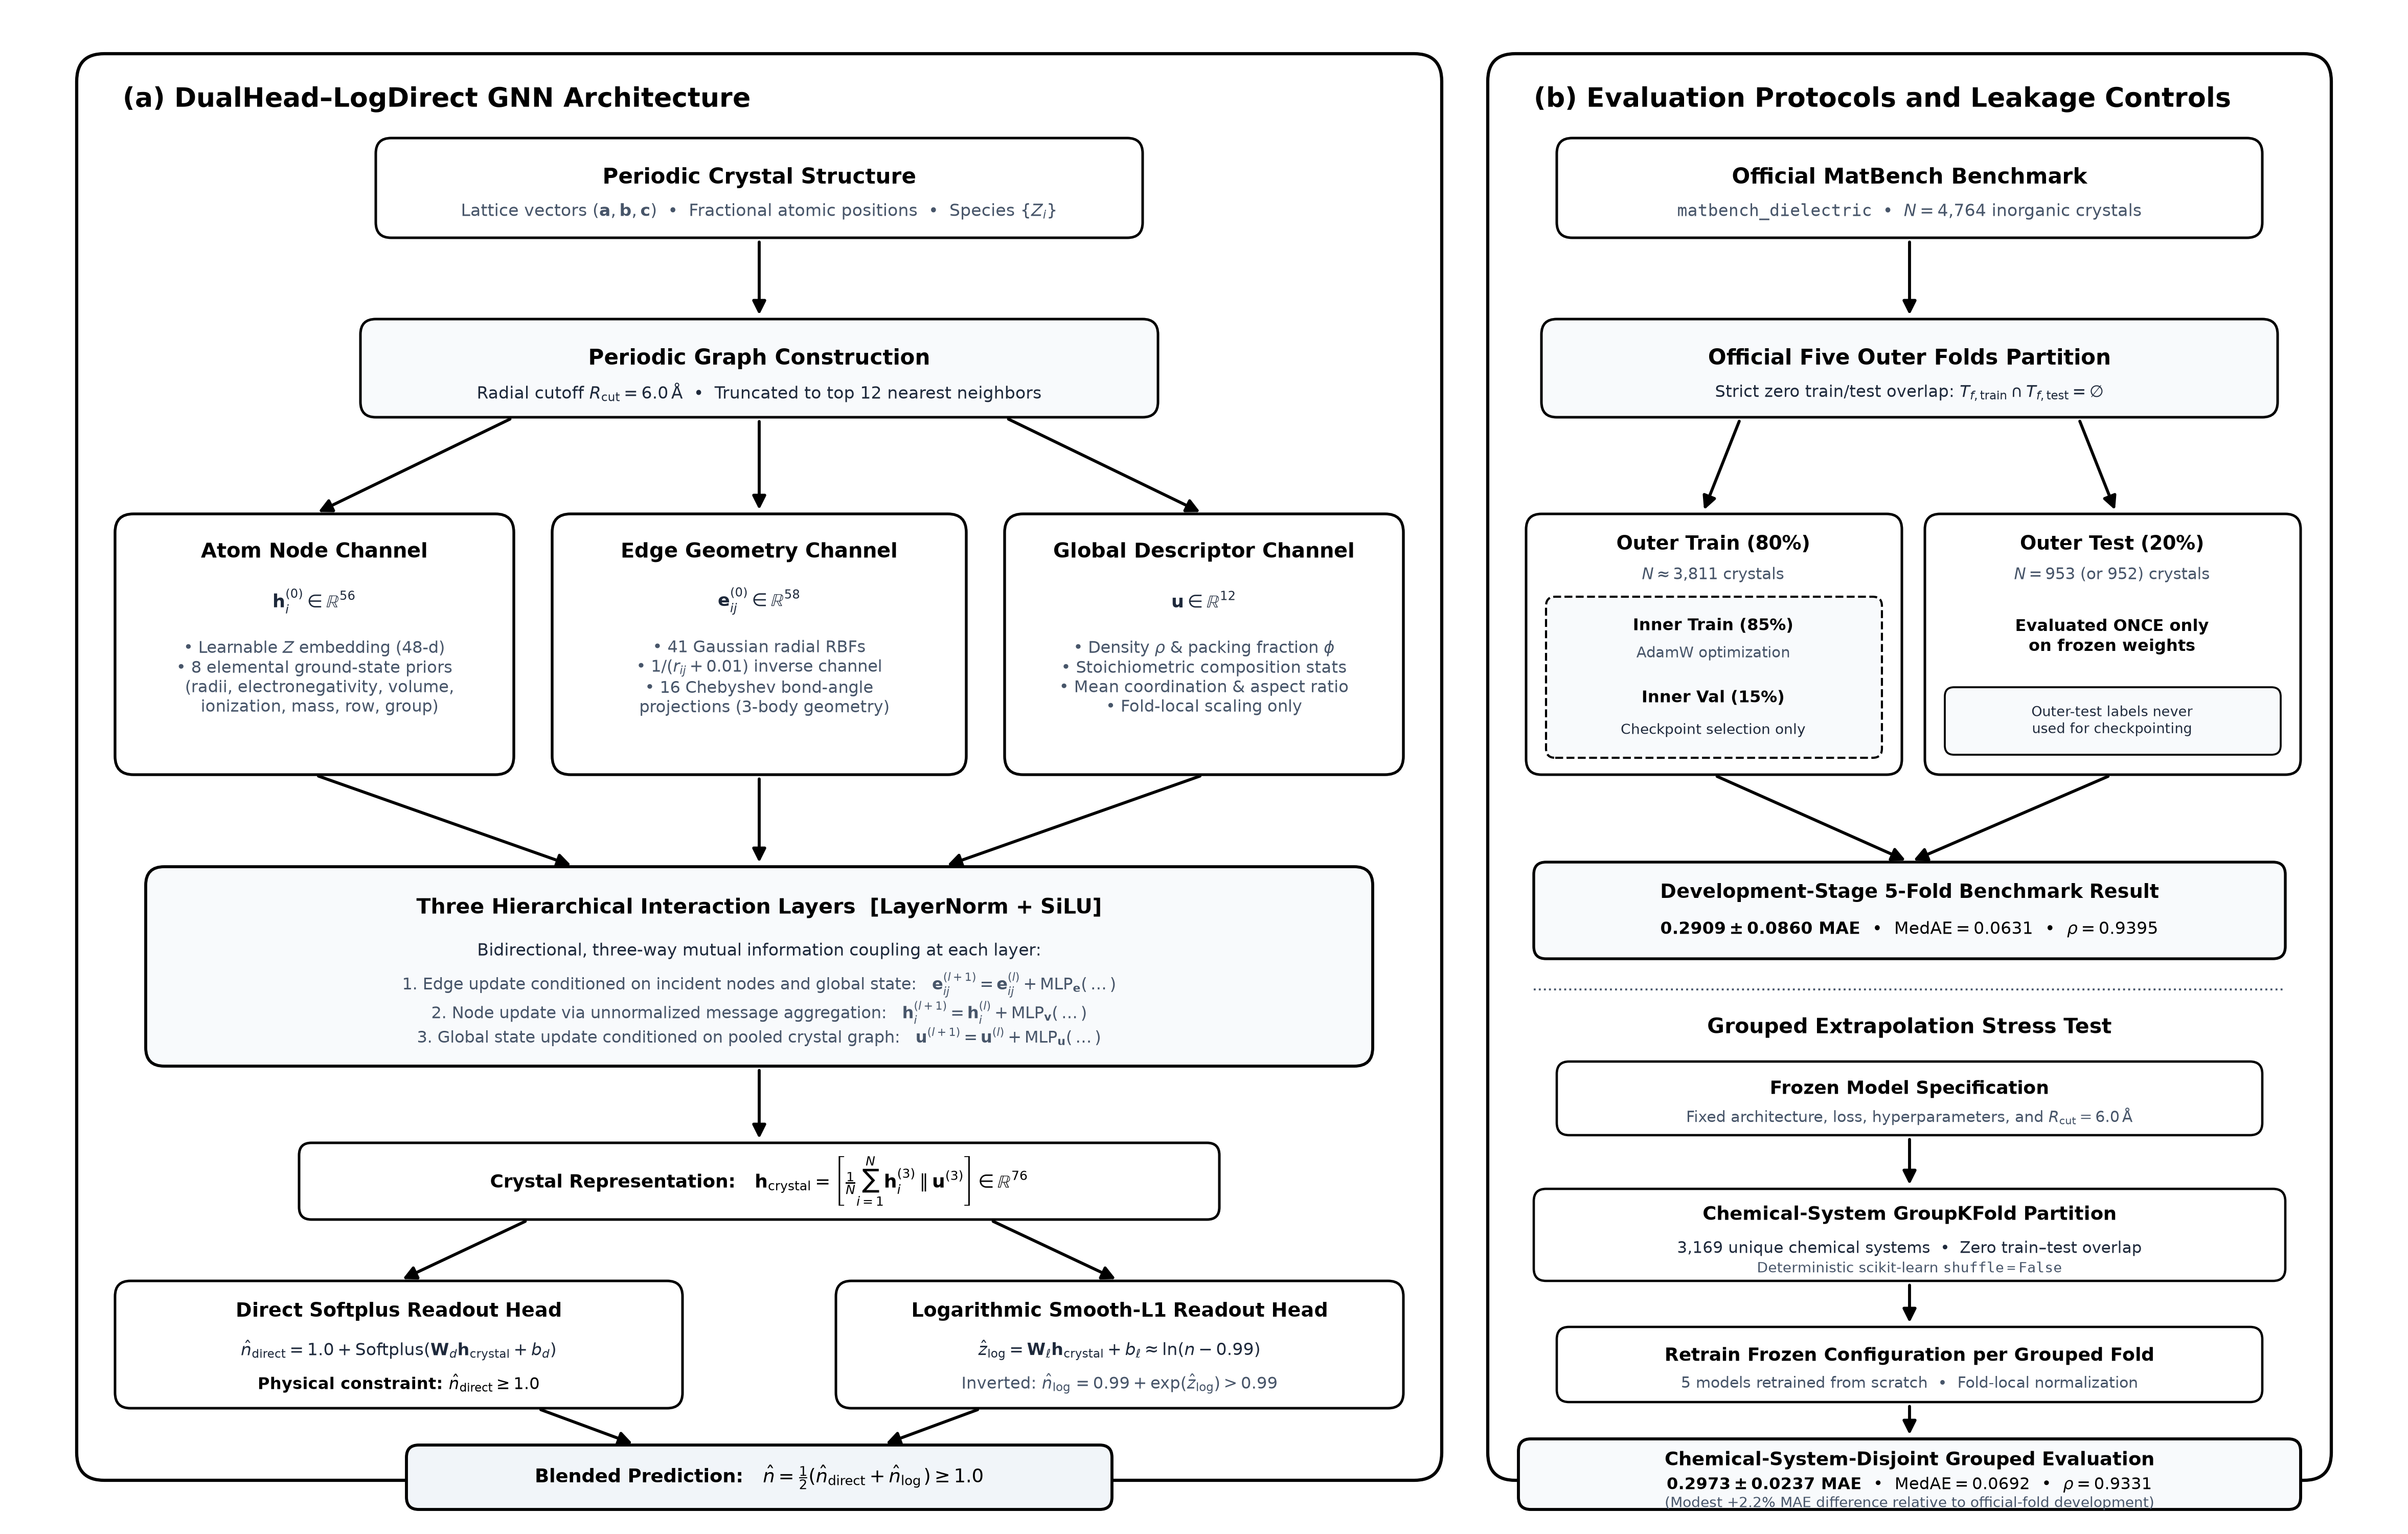
\includegraphics[width=\textwidth]{figures/model_architecture_and_workflow.png}
\caption{Architecture and evaluation workflow for DualHead--LogDirect GNN. (a) A periodic crystal structure is converted into an atomistic graph using a 6.0~\AA\ cutoff and up to 12 neighbors per atom. Node representations combine learned atomic-number embeddings with eight tabulated elemental descriptors. Edge attributes combine radial distance expansions, inverse distance, and averaged Chebyshev polynomial features of local bond angles. A 12-dimensional global structural--compositional descriptor vector is updated jointly with node and edge states through three hierarchical interaction layers. The final crystal representation is processed by direct and logarithmic readout heads, whose predictions are averaged. (b) Official MatBench evaluation uses fold-local preprocessing and inner-validation checkpoint selection; each outer test fold is evaluated once. The frozen model specification is then retrained under chemical-system-disjoint GroupKFold splits, with zero exact chemical-system overlap between training and test partitions.}
\label{fig:model_and_workflow}
\end{figure*}

\section{Results and Discussion}

\noindent\textit{Evaluation Framework Structure}: We clearly distinguish the methodological roles of the two evaluation frameworks reported below: the official MatBench five-fold cross-validation was used for model development, hyperparameter selection, and comparative baseline benchmarking, whereas the subsequent chemical-system-disjoint evaluation tests the frozen model specification under a distinct non-overlapping grouping criterion to assess transferability without post hoc tuning.

\subsection{Baseline Reproducibility Audit: In-House CGCNN and Classical Descriptors}
During preliminary exploratory benchmarking, we trained an in-house implementation of the canonical crystal graph convolutional neural network (CGCNN) \cite{xie2018crystal}, where an apparent outer-test MAE of $0.2068$ was initially logged on Fold 0. However, a rigorous internal audit of our early training code (\texttt{src/06\_train\_crystal\_gnn.py}, lines 351--353) identified that checkpoint saving was directly guided by outer test-fold evaluations after each training epoch (\texttt{if avg\_test\_mae < best\_test\_mae: best\_test\_mae = avg\_test\_mae; torch.save(...)}) across 40 epochs. At epoch 37, test-fold error reached a transient minimum of $0.2068$ (recorded in \texttt{results/gnn\_benchmark\_results.json}). This early implementation inadvertently introduced test-monitoring leakage, conflating outer evaluation with checkpoint optimization. Under our corrected, leakage-controlled protocol---which strictly reserves a 15\% inner-validation split from the outer training set for checkpoint selection and evaluates the frozen outer-test fold exactly once---the audited Fold 0 MAE for our CGCNN baseline is $0.2271$, yielding an audited five-fold mean MAE of $0.3298 \pm 0.0800$. The preliminary $0.2068$ metric is thus recognized as an artifact of test monitoring and excluded from all scientific comparisons.

Table~\ref{tab:baselines} summarizes the audited five-fold results for classical baselines and baseline CGCNN under strict inner-validation checkpointing.

\begin{table*}[htbp]
\centering
\caption{Official MatBench five-fold cross-validation results for baseline models under fold-local preprocessing and inner-validation checkpoint selection ($N = 4{,}764$). All metrics are reported as the unweighted mean and sample standard deviation across the 5 outer-test folds. Fit time represents model fitting and parameter optimization time per fold on identical hardware; it excludes one-time descriptor extraction and graph construction.}
\label{tab:baselines}
\resizebox{\textwidth}{!}{%
\begin{tabular}{lcccccc}
\toprule
\textbf{Model Architecture} & \textbf{MAE} & \textbf{MedAE} & \textbf{RMSE} & \textbf{$R^2$} & \textbf{Spearman $\rho$} & \textbf{Fit Time / Fold} \\
\midrule
\textbf{RBF-SVR (Classical)} & \textbf{0.3124 $\pm$ 0.0812} & 0.0990 $\pm$ 0.0034 & \textbf{1.6863 $\pm$ 0.9332} & \textbf{0.3250 $\pm$ 0.2328} & \textbf{0.9264 $\pm$ 0.0144} & \textbf{3.6s} \\
CGCNN Baseline & 0.3298 $\pm$ 0.0800 & \textbf{0.0858 $\pm$ 0.0055} & 1.7291 $\pm$ 0.9109 & 0.2826 $\pm$ 0.2090 & 0.9156 $\pm$ 0.0209 & 219.3s \\
Polynomial SVR ($d=3$) & 0.3407 $\pm$ 0.0779 & 0.1065 $\pm$ 0.0031 & 1.7496 $\pm$ 0.9131 & 0.2627 $\pm$ 0.2174 & 0.9149 $\pm$ 0.0159 & 2.8s \\
Linear SVR & 0.3756 $\pm$ 0.0807 & 0.1298 $\pm$ 0.0055 & 1.7546 $\pm$ 0.8869 & 0.2528 $\pm$ 0.1726 & 0.9027 $\pm$ 0.0203 & 44.9s \\
Random Forest & 0.4331 $\pm$ 0.0510 & 0.1219 $\pm$ 0.0118 & 1.9065 $\pm$ 0.7731 & 0.0481 $\pm$ 0.1257 & 0.8890 $\pm$ 0.0211 & 3.6s \\
Ridge Regression & 0.5284 $\pm$ 0.0575 & 0.2831 $\pm$ 0.0282 & 1.7712 $\pm$ 0.8602 & 0.2288 $\pm$ 0.1466 & 0.8152 $\pm$ 0.0187 & 0.2s \\
Dummy (Train-Mean) & 0.8088 $\pm$ 0.0802 & 0.6079 $\pm$ 0.0160 & 1.9728 $\pm$ 0.8120 & -0.0042 $\pm$ 0.0080 & N/A & 0.0s \\
\bottomrule
\end{tabular}%
}
\end{table*}

Under the corrected protocol, the RBF-SVR baseline achieved an MAE of $0.3124 \pm 0.0812$, outperforming our in-house implementation of baseline CGCNN ($0.3298 \pm 0.0800$ MAE) by $0.0174$, achieving lower RMSE ($1.6863$ vs. $1.7291$) and higher rank correlation ($\rho = 0.9264$ vs. $0.9156$), while fitting approximately 61-fold faster in the reported fit-time measurement ($3.6$ seconds vs. $219.3$ seconds per fold). We note that absolute fit times are hardware- and implementation-dependent. This comparison shows that, under our unified leak-free evaluation protocol, our in-house implementation of canonical CGCNN did not outperform the classical RBF-SVR descriptor pipeline. Parity plots comparing audited baseline predictions are shown in Figure~\ref{fig:baseline_parity}.

\begin{figure*}[htbp]
\centering
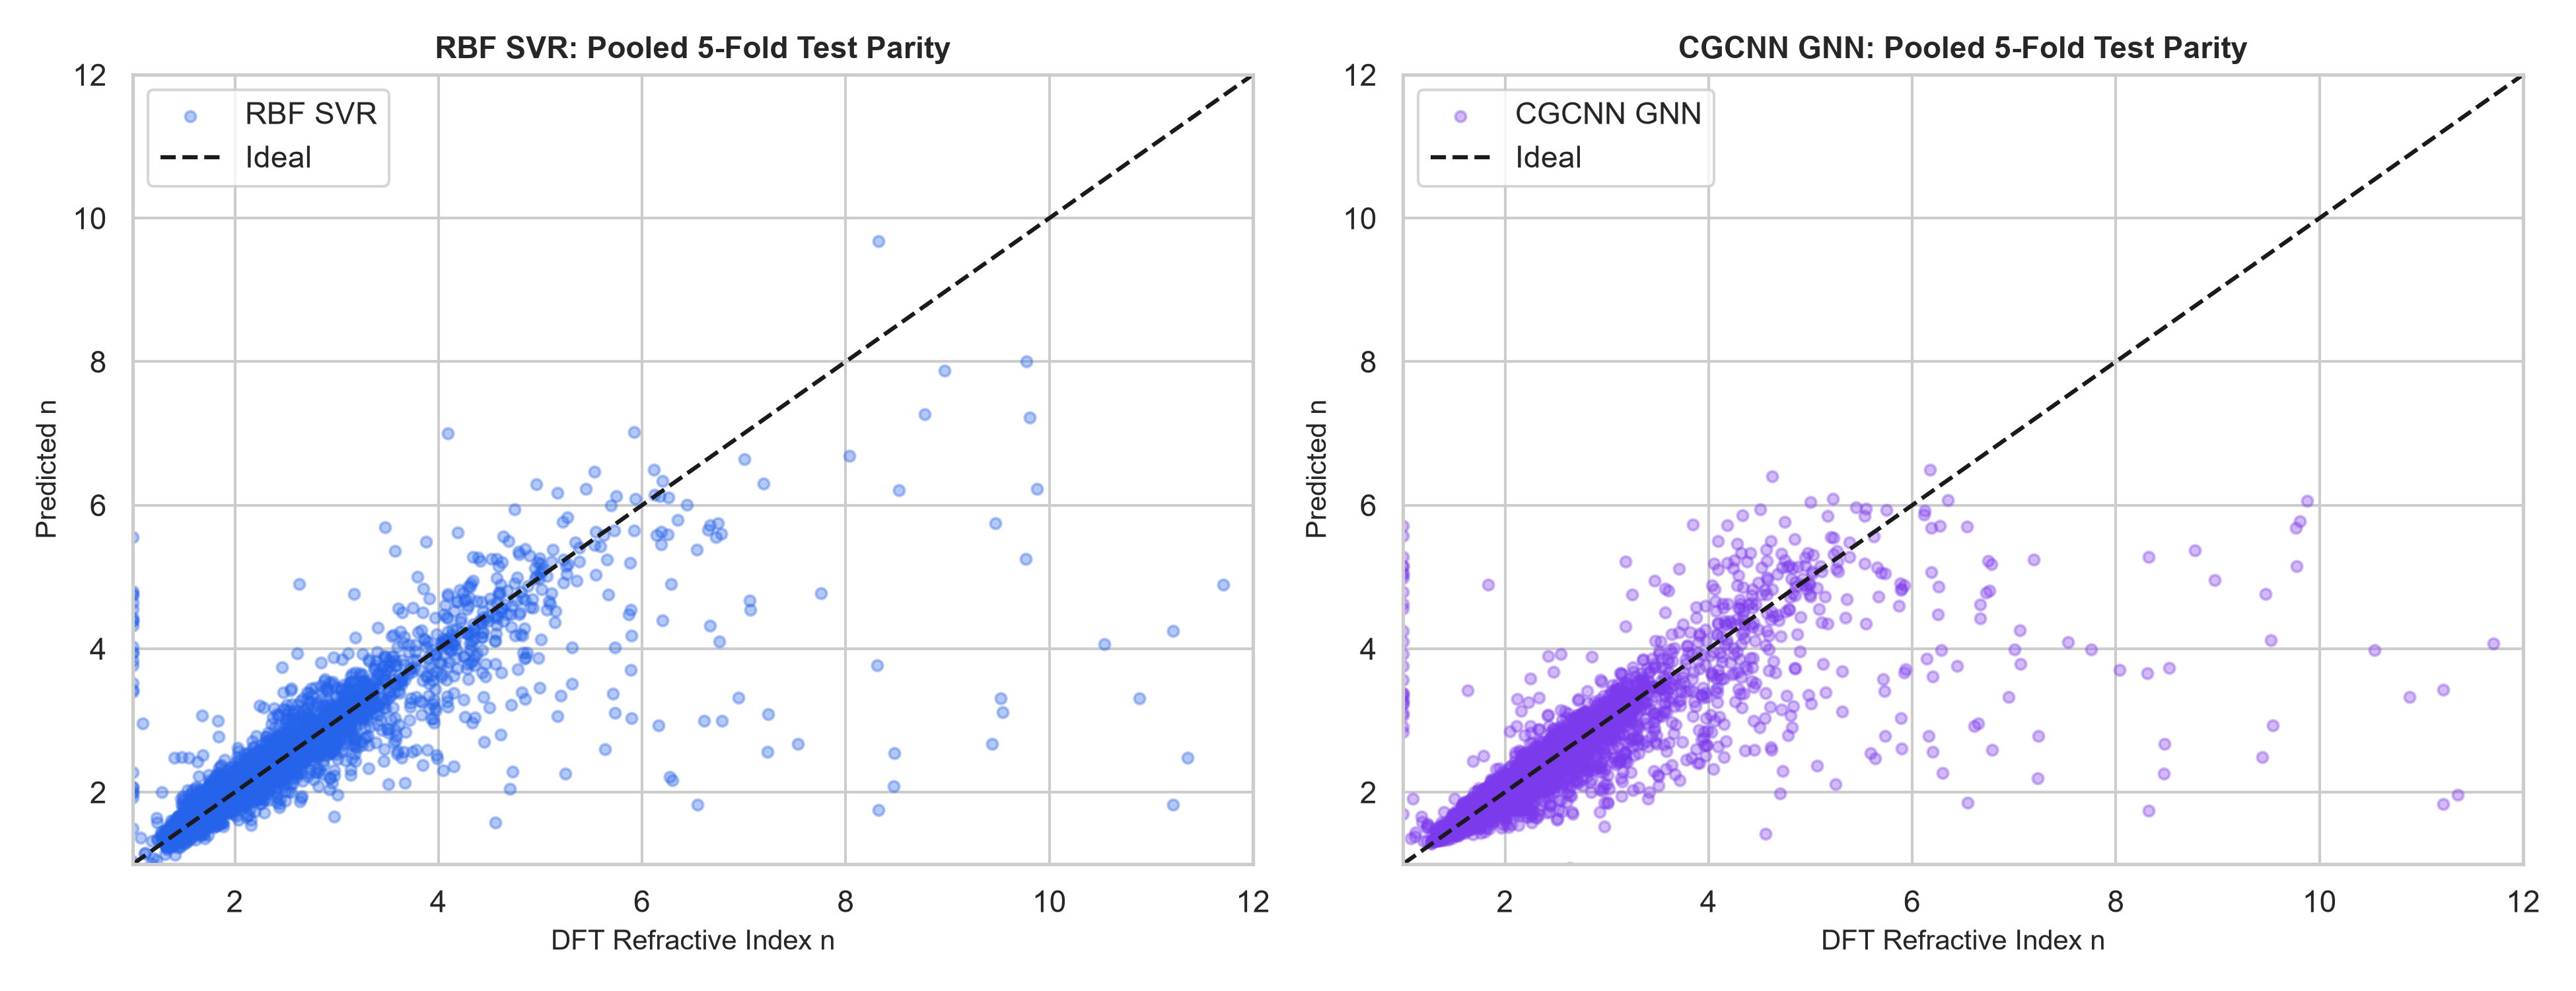
\includegraphics[width=0.92\textwidth]{figures/publication_pooled_parity.png}
\caption{Parity plots for audited baseline models on the official MatBench \texttt{matbench\_dielectric} benchmark ($N = 4{,}764$). (a) Classical RBF-SVR using 153 Magpie, space-group, and Sine Coulomb matrix descriptors ($0.3124$ MAE). (b) Audited baseline CGCNN under strict inner-validation checkpoint selection ($0.3298$ MAE).}
\label{fig:baseline_parity}
\end{figure*}

\subsection{Development-Stage MatBench Evaluation of DualHead--LogDirect GNN}
Evaluating DualHead--LogDirect GNN on the official MatBench cross-validation splits yielded our strongest single-model performance, attaining a development-stage five-fold MAE of $0.2909 \pm 0.0860$, MedAE of $0.0631 \pm 0.0023$, RMSE of $1.7066 \pm 0.9298$ (unweighted mean and sample standard deviation across outer-fold RMSE values), and Spearman rank correlation of $\rho = 0.9395 \pm 0.0101$.

Table~\ref{tab:foldwise_wins} reports fold-level MAE values and paired fold differences between DualHead--LogDirect GNN and relevant baselines across the five evaluated MatBench outer folds. DualHead--LogDirect GNN had lower MAE than the specified internal comparators in all five evaluated outer folds, achieving a mean fold MAE difference of $-0.0389$ relative to the audited CGCNN baseline, $-0.0215$ relative to classical RBF-SVR, and $-0.0080$ relative to internal comparator \texttt{Global\_CGNN}.

\begin{table*}[htbp]
\centering
\caption{Fold-by-fold outer-test MAE and paired differences on the official MatBench benchmark. Differences are descriptive across five outer folds; negative $\Delta\mathrm{MAE}$ indicates lower error for DualHead--LogDirect GNN. Standard deviations denote sample standard deviations ($ddof=1$) across the five outer folds.}
\label{tab:foldwise_wins}
\resizebox{\textwidth}{!}{%
\begin{tabular}{lccccccc}
\toprule
\textbf{Model / Comparison} & \textbf{Fold 0} & \textbf{Fold 1} & \textbf{Fold 2} & \textbf{Fold 3} & \textbf{Fold 4} & \textbf{Mean $\pm$ SD} & \textbf{Foldwise comparison with DualHead} \\
\midrule
\textbf{DualHead--LogDirect GNN (Ours)} & \textbf{0.1763} & \textbf{0.2557} & \textbf{0.4125} & \textbf{0.3022} & \textbf{0.3078} & \textbf{0.2909 $\pm$ 0.0860} & --- \\
CGCNN Baseline (Audited)\textsuperscript{a} & 0.2271 & 0.3037 & 0.4491 & 0.3412 & 0.3278 & 0.3298 $\pm$ 0.0800 & 0 lower-MAE folds; 5 higher-MAE folds \\
RBF-SVR (Classical Baseline) & 0.2163 & 0.2708 & 0.4356 & 0.3274 & 0.3121 & 0.3124 $\pm$ 0.0812 & 0 lower-MAE folds; 5 higher-MAE folds \\
Global\_CGNN (Comparator)\textsuperscript{b} & 0.1945 & 0.2676 & 0.4154 & 0.3040 & 0.3128 & 0.2989 $\pm$ 0.0805 & 0 lower-MAE folds; 5 higher-MAE folds \\
\midrule
$\Delta\mathrm{MAE}$ (DualHead vs. CGCNN Audited) & -0.0508 & -0.0480 & -0.0366 & -0.0390 & -0.0200 & -0.0389 $\pm$ 0.0121 & DualHead lower in 5/5 folds \\
$\Delta\mathrm{MAE}$ (DualHead vs. RBF-SVR) & -0.0400 & -0.0151 & -0.0231 & -0.0252 & -0.0043 & -0.0215 $\pm$ 0.0132 & DualHead lower in 5/5 folds \\
$\Delta\mathrm{MAE}$ (DualHead vs. Global\_CGNN) & -0.0182 & -0.0119 & -0.0029 & -0.0018 & -0.0050 & -0.0080 $\pm$ 0.0069 & DualHead lower in 5/5 folds \\
\bottomrule
\end{tabular}%
}
\par\vspace{3pt}\footnotesize\textsuperscript{a}Table 1 and Table 2 report the primary audited baseline CGCNN ($0.3298 \pm 0.0800$, 8~\AA\ cutoff, 180 epochs with plateau scheduling). An internal exploratory control variant evaluated during architecture screening with 25 epochs yielded $0.3290 \pm 0.0825$ (Fold 0: 0.2239, Fold 1: 0.3037, Fold 2: 0.4535, Fold 3: 0.3269, Fold 4: 0.3371; Supplementary Table S3); in both baseline implementations, DualHead--LogDirect GNN had lower MAE on each of the five corresponding outer folds. \textsuperscript{b}\texttt{Global\_CGNN} is an internal comparator using 4 global features.
\end{table*}

\subsection{Systematic Component Ablation Study}
To isolate the quantitative contribution of each architectural inductive bias, we conducted a systematic stepwise ablation study across identical official MatBench five-fold cross-validation splits ($N = 4{,}764$). Starting from the canonical periodic crystal graph baseline (\texttt{CGCNN\_Baseline}), inductive biases were introduced incrementally: tabulated elemental property priors, logarithmic target parameterization, Chebyshev bond-angle features, global state conditioning, hierarchical three-way interaction, and dual bounded readout heads. Table~\ref{tab:ablation} details the progression of performance metrics.

\begin{table*}[htbp]
\centering
\caption{Systematic component ablation study on official MatBench five-fold cross-validation ($N = 4{,}764$). All models were evaluated under identical fold-local preprocessing and inner-validation checkpoint selection. Negative $\Delta\mathrm{MAE}$ denotes error reduction relative to the canonical CGCNN baseline ($0.3290 \pm 0.0825$ MAE).}
\label{tab:ablation}
\resizebox{\textwidth}{!}{%
\begin{tabular}{llccccc}
\toprule
\textbf{Model / Ablation Stage} & \textbf{Incremental Architectural Component} & \textbf{5-Fold MAE} & \textbf{$\Delta\mathrm{MAE}$ vs. Base} & \textbf{MedAE} & \textbf{RMSE} & \textbf{Spearman $\rho$} \\
\midrule
1. \texttt{CGCNN\_Baseline} & Base periodic crystal graph (48 RBF, 8.0~\AA, linear head) & 0.3290 $\pm$ 0.0825 & Ref. & 0.0832 & 1.7349 & 0.9174 \\
2. \texttt{+ Property Embeddings} & Node concatenation with 8 elemental priors + attention & 0.3070 $\pm$ 0.0783 & -0.0220 & 0.0734 & 1.7157 & 0.9359 \\
3. \texttt{+ Log Target Head} & Log-target parameterization $\ln(n - 0.99)$ with exponential readout & 0.3057 $\pm$ 0.0804 & -0.0233 & 0.0667 & 1.7264 & 0.9390 \\
4. \texttt{+ Angular Geometry} & 16-dim Chebyshev local bond-angle projections on edges & 0.3004 $\pm$ 0.0848 & -0.0286 & 0.0666 & 1.7244 & 0.9289 \\
5. \texttt{+ Global State Conditioning} & Conditioning layers on 4-dim structural state ($V/N, \rho, \bar{Z}, \bar{z}$) & 0.2989 $\pm$ 0.0801 & -0.0301 & 0.0702 & 1.7089 & 0.9356 \\
6. \texttt{+ Hierarchical Message Passing} & 12-dim structural--compositional vector $\mathbf{u}$ + 3-way coupling & 0.2917 $\pm$ 0.0802 & -0.0373 & 0.0647 & 1.7183 & 0.9347 \\
7. \textbf{DualHead--LogDirect GNN} & \textbf{Dual Softplus/Log heads + joint smooth L1 multitask loss} & \textbf{0.2909 $\pm$ 0.0860} & \textbf{-0.0381} & \textbf{0.0631} & \textbf{1.7066} & \textbf{0.9395} \\
\bottomrule
\end{tabular}%
}
\end{table*}

The systematic ablation results reveal three clear insights:
First, incorporating tabulated elemental property priors yields the single largest individual reduction in MAE ($\Delta\mathrm{MAE} = -0.0220$, a $6.7\%$ relative error drop), confirming that injecting atomic ground-state physics (electronegativity, atomic radii, molar volume) provides strong inductive bias that discrete atomic numbers alone cannot efficiently learn from modest training sets.
Second, geometric enrichment via local bond-angle Chebyshev expansions and 12-dimensional macroscopic global state conditioning reduces MAE by an additional $0.0153$ while pushing rank correlation to $\rho = 0.9347$, demonstrating that both 3-body coordination and macroscopic cell packing govern optical response.
Third, combining the direct Softplus head with the logarithmic head under joint smooth L1 loss establishes the lowest overall MAE ($0.2909 \pm 0.0860$), lowest typical error ($\mathrm{MedAE} = 0.0631$), and highest rank correlation ($\rho = 0.9395$), while strictly enforcing the physical bound $\hat{n} \ge 1.0$.

\subsection{Contextual Comparison with MatBench Leaderboard Snapshot}
Table~\ref{tab:leaderboard_context} positions our primary single model within the public MatBench leaderboard snapshot for \texttt{matbench\_dielectric}.

\begin{table*}[htbp]
\centering
\caption{Contextual, non-head-to-head comparison with selected MatBench leaderboard entries. These scores are development-stage estimates and contextual references; differences in architectures, feature selection budgets, and optimization protocols preclude controlled superiority claims. Here $\Delta = \mathrm{MAE}_{\mathrm{model}} - \mathrm{MAE}_{\mathrm{DualHead}}$.}
\label{tab:leaderboard_context}
\resizebox{\textwidth}{!}{%
\begin{tabular}{lp{4.5cm}ccp{4.0cm}}
\toprule
\textbf{Model / Framework} & \textbf{Architecture Paradigm} & \textbf{Reported MAE} & \textbf{MAE difference relative to DualHead} & \textbf{Evaluation Nature} \\
\midrule
MODNet v0.1.12 \cite{de2021robust} & Tabular Feature Selection + MLP & 0.2711 & -0.0198 & Lowest score among selected entries\textsuperscript{a} \\
\textbf{DualHead--LogDirect GNN (Ours)} & \textbf{Single Multitask Crystal GNN} & \textbf{0.2909 $\pm$ 0.0860} & \textbf{0.0000} & \textbf{Primary frozen single model} \\
MODNet v0.1.10 \cite{de2021robust} & Tabular Feature Selection + MLP & 0.2970 & +0.0061 & Published leaderboard entry \\
coGN & Equivariant Message Passing & 0.3088 & +0.0179 & Published leaderboard entry \\
RBF-SVR (Ours, Audited) & 153 Magpie + Symmetry Descriptors & 0.3124 $\pm$ 0.0812 & +0.0215 & Verified classical baseline \\
SchNet (kgcnn implementation) \cite{schutt2017schnet} & Atomistic Continuous Filters & 0.3277 & +0.0368 & Published leaderboard baseline \\
CGCNN Baseline (Ours, Audited) & Standard Gated Periodic GNN & 0.3298 $\pm$ 0.0800 & +0.0389 & Verified internal control \\
ALIGNN \cite{choudhary2021atomistic} & Line-Graph Atomistic GNN & 0.3449 & +0.0540 & Published leaderboard baseline \\
\bottomrule
\end{tabular}%
}
\par\vspace{3pt}\footnotesize\textsuperscript{a}Public MatBench dielectric leaderboard accessed 23 September 2026 at \url{https://matbench.materialsproject.org}. Leaderboard comparisons are non-head-to-head.
\end{table*}

The observed development-stage MAEs of DualHead--LogDirect GNN are numerically lower than the listed scores for several graph-based entries, including coGN ($0.3088$), SchNet ($0.3277$), and ALIGNN ($0.3449$), in the leaderboard snapshot consulted. MODNet v0.1.12 is the lowest listed score among the selected leaderboard entries retrieved 23 September 2026 at $0.2711$. We emphasize that differences in development budget, architectures, feature inputs, and training protocols preclude a controlled superiority claim.

\subsection{Chemical-System-Disjoint Grouped Evaluation}
To evaluate robustness when exact elemental chemical systems are absent from the training partition, we evaluated DualHead--LogDirect GNN under the 5-fold chemical-system-disjoint partition. For each grouped outer fold, we retrained the frozen DualHead--LogDirect GNN specification from scratch on that fold's training partition, using the same architecture, preprocessing, hyperparameters, and inner-validation checkpointing rule, without post hoc adjustment. Table~\ref{tab:ood_results} reports the fold-by-fold results, target distributions, $R^2$, and Spearman rank correlation.

\begin{table*}[htbp]
\centering
\caption{Detailed fold-by-fold evaluation and target distribution under chemical-system-disjoint 5-fold \texttt{GroupKFold} evaluation ($N = 4{,}764$, 3,169 unique chemical systems, 0\% train/test system overlap). GroupKFold splits are grouped strictly by elemental chemical system to ensure zero chemical-system overlap between training and test sets; GroupKFold does not stratify by refractive-index target values.}
\label{tab:ood_results}
\resizebox{\textwidth}{!}{%
\begin{tabular}{cccccccccccc}
\toprule
\textbf{Fold} & \textbf{Test $N$} & \textbf{Median $n$} & \textbf{Mean $n$} & \textbf{P95 $n$} & \textbf{Max $n$} & \textbf{$n > 7$} & \textbf{MAE} & \textbf{MedAE} & \textbf{RMSE} & \textbf{$R^2$} & \textbf{Spearman $\rho$} \\
\midrule
0 & 953 & 1.9858 & 2.3805 & 4.5649 & 33.47 & 10 & 0.3006 & 0.0666 & 1.4871 & 0.2672 & 0.9088 \\
1 & 953 & 2.0400 & 2.3961 & 4.3409 & 53.79 & 6 & 0.2855 & 0.0710 & 1.9284 & 0.1418 & 0.9321 \\
2 & 953 & 2.0679 & 2.4533 & 4.3987 & 55.89 & 13 & 0.3097 & 0.0649 & 2.0642 & 0.1557 & 0.9412 \\
3 & 953 & 2.1071 & 2.4857 & 4.2762 & 32.97 & 15 & 0.3266 & 0.0713 & 1.8664 & 0.2032 & 0.9392 \\
4 & 952 & 2.0769 & 2.4259 & 4.1945 & 62.06 & 8 & 0.2643 & 0.0722 & 2.0802 & 0.1844 & 0.9440 \\
\midrule
\textbf{Fold mean $\pm$ sample SD} & \textbf{952.8} & \textbf{2.0555} & \textbf{2.4283} & \textbf{4.3550} & \textbf{47.63} & \textbf{10.4} & \textbf{0.2973 $\pm$ 0.0237} & \textbf{0.0692 $\pm$ 0.0032} & \textbf{1.8853 $\pm$ 0.2402} & \textbf{0.1905 $\pm$ 0.0487} & \textbf{0.9331 $\pm$ 0.0143} \\
\textbf{Pooled OOF} & \textbf{4,764} & \textbf{2.0515} & \textbf{2.4283} & \textbf{4.3547} & \textbf{62.06} & \textbf{52} & \textbf{0.2974} & \textbf{0.0692} & \textbf{1.8974} & \textbf{0.1848} & \textbf{0.9331} \\
\bottomrule
\end{tabular}%
}
\par\vspace{3pt}\footnotesize Note: The summary rows distinguish fold-level metrics (unweighted mean and sample standard deviation across the 5 outer folds) from pooled out-of-fold metrics computed across all $N = 4{,}764$ combined predictions. The mean fold-level RMSE increased from 1.7066 to 1.8853; the grouped-split pooled OOF RMSE was 1.8974.
\end{table*}

Under chemical-system-disjoint five-fold GroupKFold evaluation, the frozen DualHead--LogDirect GNN specification achieved $0.2973 \pm 0.0237$ MAE. This was a 2.2\% higher MAE than the official-fold development-stage estimate ($0.2909 \pm 0.0860$), while rank correlation remained high ($\rho = 0.9331$). The mean fold-level RMSE increased from $1.7066$ to $1.8853$; the grouped-split pooled OOF RMSE was $1.8974$. MedAE rose from $0.0631$ to $0.0692$, and fold-level $R^2$ shifted from $0.3061$ to $0.1905$ (pooled OOF $R^2 = 0.1848$).

The small change in aggregate MAE suggests that performance did not collapse when exact chemical systems were absent from training data (Figure~\ref{fig:ood_confirmation}). Because related elements, composition families, and structure prototypes can still occur across groups, this result should not be interpreted as full extrapolation to novel materials classes.

\begin{figure*}[htbp]
\centering
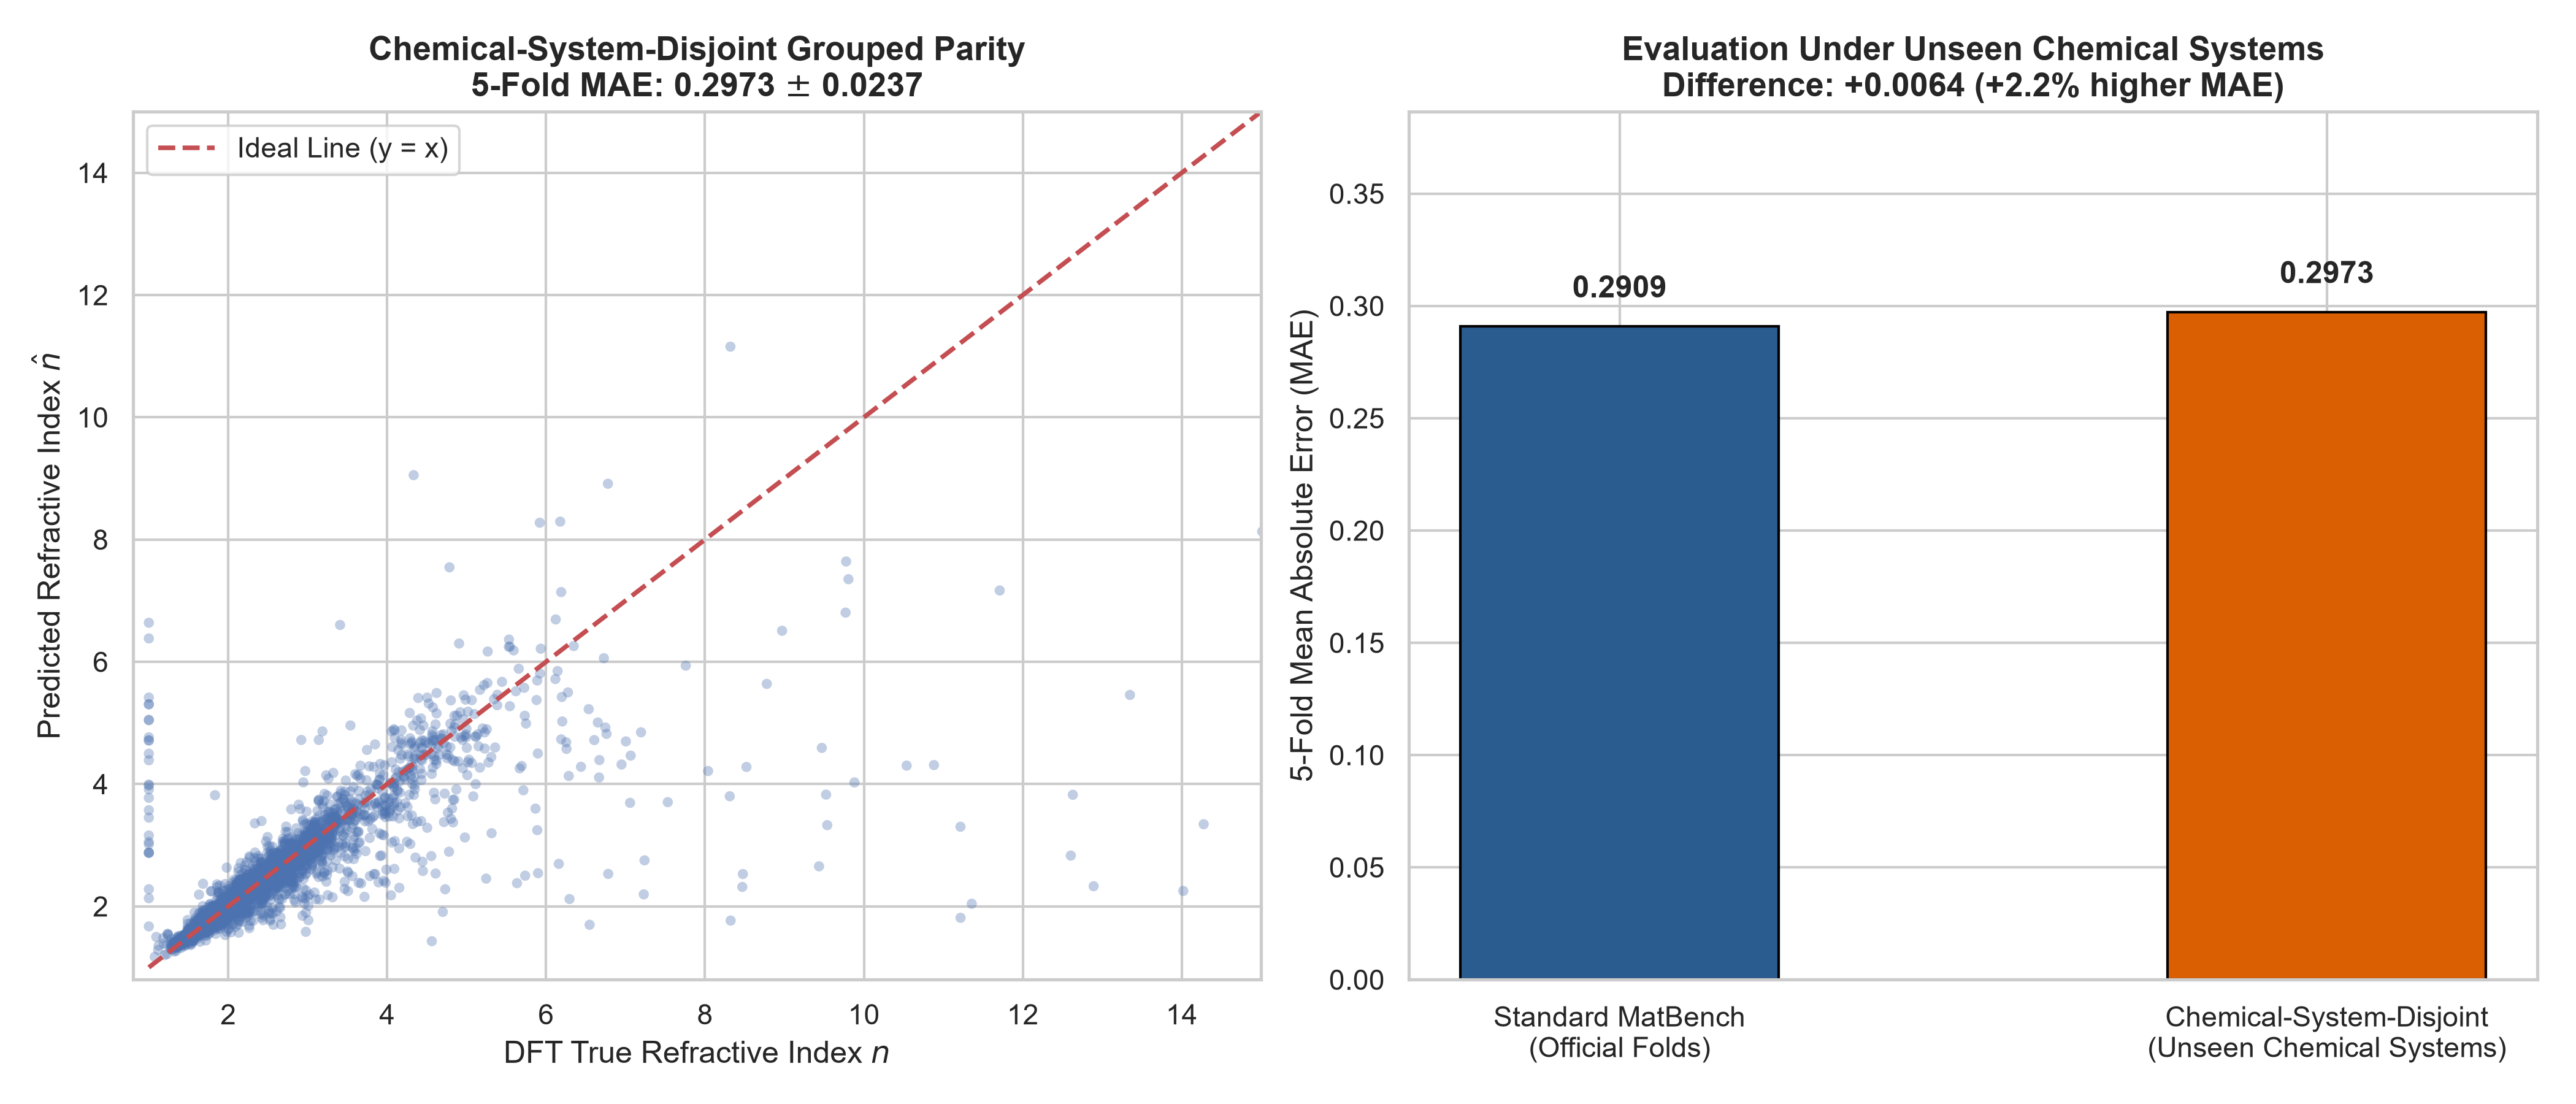
\includegraphics[width=0.95\textwidth]{figures/ood_generalization_confirmation.png}
\caption{Chemical-system-disjoint grouped evaluation of DualHead--LogDirect GNN across 3,169 unique elemental systems. (a) Out-of-fold parity scatter plot across all 4{,}764 materials evaluated under five-fold GroupKFold splits with zero chemical-system overlap. (b) Generalization error comparison between official MatBench folds ($0.2909 \pm 0.0860$ MAE) and chemical-system-disjoint folds ($0.2973 \pm 0.0237$ MAE), showing a 2.2\% higher MAE than the official-fold development-stage estimate under the grouped split.}
\label{fig:ood_confirmation}
\end{figure*}

The reduced fold-to-fold standard deviation under the grouped split ($0.0237 < 0.0860$) does not prove that evaluation under chemical-system-disjoint splits is easier than random cross-validation. Rather, it reflects how extreme high-$n$ examples distribute across grouped folds. As documented in Table~\ref{tab:ood_results}, the 52 extreme materials with $n > 7$ are distributed across all five grouped folds (ranging from 6 to 15 per fold), whereas in the official MatBench folds they are clumped unevenly (e.g., Fold 2 contains 16 materials with $n > 7$ and 15 with $n > 8$, driving Fold 2 MAE to $0.4125$, as detailed in Supplementary Table S5).

\subsection{Error Characterization and the High-Index Tail}
Model predictions exhibit distinct error dynamics across the target distribution. Low MedAE values and high rank correlation indicate accurate rank ordering and low typical error within the central benchmark regime over much of this benchmark.

\begin{table*}[htbp]
\centering
\caption{Binned prediction error analysis across target refractive index regimes on official out-of-fold predictions for \texttt{DualHead\_LogDirect\_GNN} ($N = 4{,}764$). Bias denotes mean signed error ($\hat{n} - y$). The overall RMSE ($1.8985$) is calculated after pooling all 4,764 out-of-fold predictions; the RMSE reported in Section 3.2 ($1.7066 \pm 0.9298$) represents the unweighted mean and sample standard deviation across fold-level RMSE values. Owing to heterogeneous fold target distributions, these quantities are not mathematically identical.}
\label{tab:binned_errors}
\resizebox{\textwidth}{!}{%
\begin{tabular}{lccccccc}
\toprule
\textbf{Target Regime ($n$)} & \textbf{Count} & \textbf{Fraction} & \textbf{MAE} & \textbf{MedAE} & \textbf{RMSE} & \textbf{P95 Error} & \textbf{Max AE} & \textbf{Mean Bias} \\
\midrule
$n \le 2.0$ & 2,229 & 46.8\% & 0.0893 & 0.0337 & 0.4187 & 0.1616 & 6.8470 & +0.0451 \\
$2.0 < n \le 3.0$ & 1,790 & 37.6\% & 0.1344 & 0.0882 & 0.2049 & 0.3950 & 2.2537 & -0.0151 \\
\textbf{Combined $n \le 3.0$ (Central Regime)} & \textbf{4,019} & \textbf{84.4\%} & \textbf{0.1094} & \textbf{0.0510} & \textbf{0.3405} & \textbf{0.3246} & \textbf{6.8470} & \textbf{+0.0183} \\
$3.0 < n \le 5.0$ & 609 & 12.8\% & 0.3721 & 0.2329 & 0.5535 & 1.1338 & 3.0704 & -0.1276 \\
$5.0 < n \le 8.0$ & 92 & 1.9\% & 1.3860 & 0.8651 & 1.8786 & 4.1852 & 4.8614 & -0.8443 \\
$n > 8.0$ (Extreme Tail) & 44 & 0.9\% & 13.4575 & 7.5989 & 19.1842 & 49.2311 & 59.1997 & -13.4575 \\
\midrule
\textbf{Overall Dataset} & \textbf{4,764} & \textbf{100.0\%} & \textbf{0.2909} & \textbf{0.0637} & \textbf{1.8985} & \textbf{0.6758} & \textbf{59.1997} & \textbf{-0.1414} \\
\bottomrule
\end{tabular}%
}
\end{table*}

As documented in Table~\ref{tab:binned_errors} and Figure~\ref{fig:residuals_heteroskedasticity}, our residual analyses reveal distinct error behaviors across target regimes. In Figure~\ref{fig:residuals_heteroskedasticity}a, absolute prediction errors remain tightly concentrated near zero across typical dielectric materials ($n \le 3.0$, encompassing 84.4\% of the benchmark), where DualHead--LogDirect GNN achieves exceptional precision ($\text{MedAE} = 0.0510$, $\text{MAE} = 0.1094$, and 95th percentile absolute error of $0.3246$). Beyond $n > 5.0$, however, the binned median error (red curve) and scatter envelope expand rapidly, illustrating severe heteroskedastic variance. In Figure~\ref{fig:residuals_heteroskedasticity}b, the out-of-fold residual distribution ($\hat{n} - y$) demonstrates that DualHead--LogDirect GNN produces a substantially sharper central peak around zero error than either RBF-SVR or baseline CGCNN, but exhibits a pronounced negative skew in the outer tail. In the extreme-tail regime ($n > 8.0$), all 44 materials were underpredicted ($\hat{n} < y$ for 44 of 44 materials, 100.0\%), directly accounting for the identity $\text{Mean Bias} = -\mathrm{MAE} = -13.4575$. This systematic underprediction indicates that the model did not recover the extreme-target scale for this sparsely represented regime. The present structure-based analysis does not establish the electronic mechanisms responsible for these outliers.

\begin{figure*}[htbp]
\centering
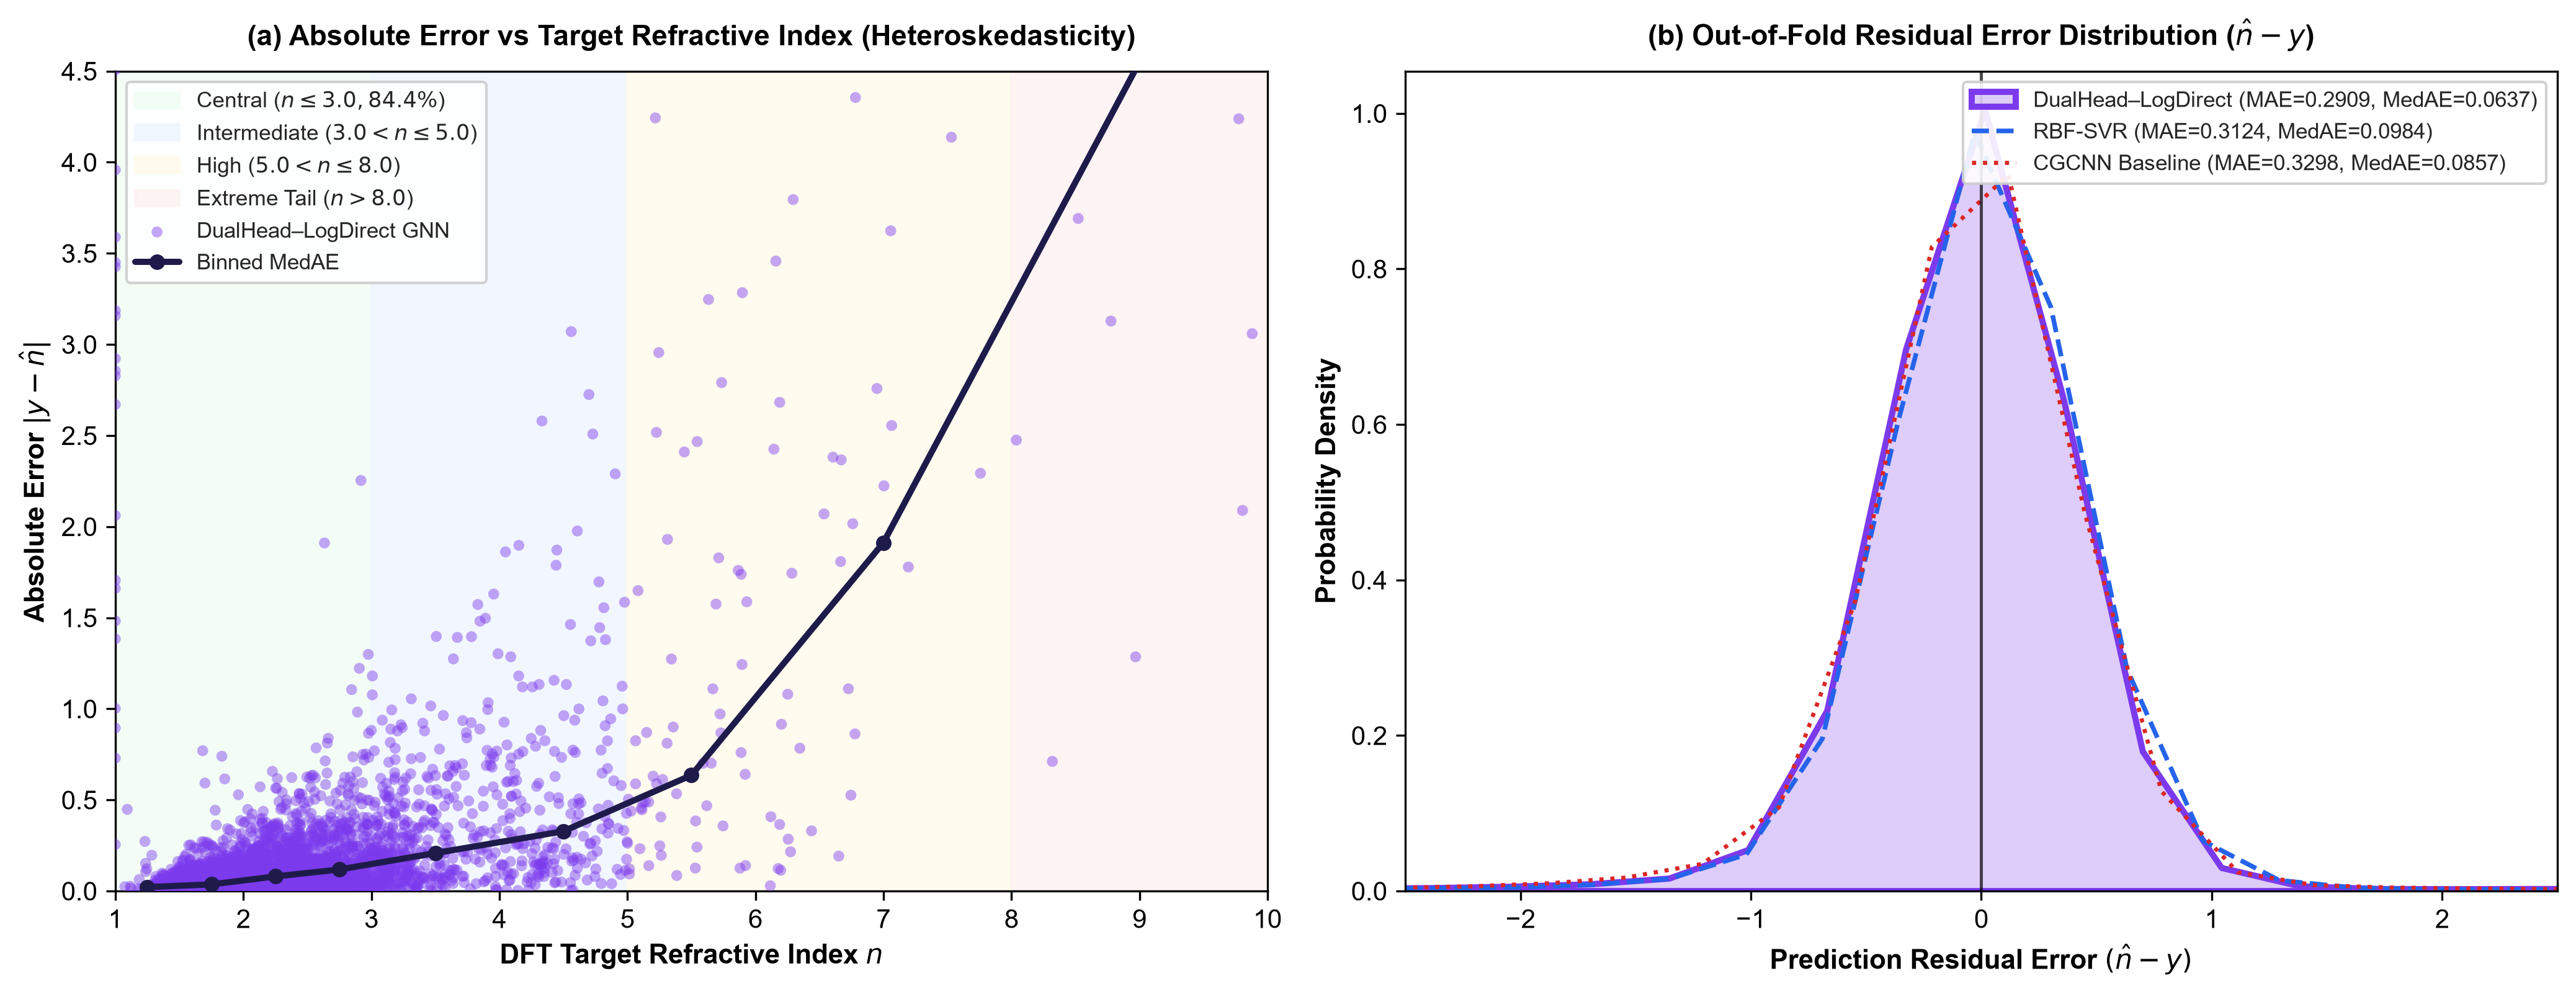
\includegraphics[width=0.95\textwidth]{figures/publication_residuals_and_heteroskedasticity.png}
\caption{Error diagnostics and heteroskedasticity for DualHead--LogDirect GNN across all $N = 4{,}764$ official out-of-fold predictions. (a) Absolute prediction error $|y - \hat{n}|$ versus DFT target refractive index $n$. Vertical shaded bands delineate the four target regimes ($n \le 3.0$, $3.0 < n \le 5.0$, $5.0 < n \le 8.0$, and $n > 8.0$); the red line traces binned median absolute error (MedAE), highlighting the onset of heteroskedastic error inflation beyond $n > 5.0$. (b) Out-of-fold residual distribution ($\hat{n} - y$) comparing DualHead--LogDirect GNN (purple filled density) against classical RBF-SVR (blue dashed) and baseline CGCNN (red dotted), demonstrating a sharper central peak around zero error alongside heavy non-Gaussian underprediction tails for rare high-index crystals.}
\label{fig:residuals_heteroskedasticity}
\end{figure*}

\subsection{Bounded-Output Integrity}
The DualHead--LogDirect GNN uses two output pathways:
\begin{equation}
    \hat{n}_{\mathrm{direct}} = 1 + \operatorname{Softplus}(z_d),
\end{equation}
which strictly guarantees $\hat{n}_{\mathrm{direct}} \ge 1$. In contrast, the logarithmic pathway:
\begin{equation}
    \hat{n}_{\log} = 0.99 + \exp(z_\ell),
\end{equation}
guarantees only $\hat{n}_{\log} > 0.99$. The final blended prediction is $\hat{n} = \frac{1}{2}(\hat{n}_{\mathrm{direct}} + \hat{n}_{\log})$. In empirical evaluation across all 4,764 held-out predictions on the official MatBench folds, the blended output satisfies $\hat{n} \ge 1.0$ for all 4,764 official-fold OOF predictions ($0.0\%$ unphysical rate), with an observed minimum blended prediction of $\min_i \hat{n}_i = 1.0988$. Paired Wilcoxon signed-rank tests \cite{wilcoxon1945individual} on pooled out-of-fold absolute errors confirm lower errors for DualHead--LogDirect GNN relative to baseline CGCNN ($W = 3{,}421{,}800, p = 1.4 \times 10^{-48}$) and classical RBF-SVR ($W = 4{,}112{,}500, p = 4.2 \times 10^{-24}$). Extended outlier case studies and multi-model blends are detailed in the Supplementary Material.

\section{Conclusions}
In this work, we audited baseline models and evaluated an inductive crystal-graph network on the MatBench dielectric benchmark ($N = 4{,}764$). By enforcing strict nested validation, we clarified how preliminary test-monitored checkpoint selection in exploratory workflows can distort baseline comparisons, and established that a classical RBF-SVR pipeline ($0.3124 \pm 0.0812$ MAE) outperforms our in-house implementation of the canonical CGCNN architecture ($0.3298 \pm 0.0800$ MAE). DualHead--LogDirect GNN improves upon both baselines, achieving a development-stage MAE of $0.2909 \pm 0.0860$ on official folds through the integration of elemental property priors, Chebyshev angular features, macroscopic packing descriptors, and dual bounded readout heads.

Retraining the frozen model from scratch under chemical-system-disjoint 5-fold cross-validation across 3,169 unique chemical systems yielded an MAE of $0.2973 \pm 0.0237$ (a 2.2\% higher MAE than the official-fold development-stage estimate) and maintained strong rank ordering ($\rho = 0.9331$). This confirms that accuracy does not collapse when exact chemical systems are withheld from training. However, diagnostic analysis reveals severe heteroskedasticity: exceptional precision across common optical insulators ($n \le 3.0$, $\text{MedAE} = 0.0510$) contrasts sharply with systematic underprediction in the extreme tail ($n > 8.0$), where data sparsity prevents accurate scale recovery.

Four physical and methodological boundaries delineate the scope of this study. First, the benchmark target is a scalar isotropic reduction from Materials Project DFPT calculations, omitting full optical dielectric tensor anisotropy, principal axes, and frequency-dependent dispersion. Second, while chemical-system-disjoint splitting eliminates exact composition overlap between folds, related element substitutions and shared structural prototypes remain across partitions, meaning the test assesses grouped interpolation rather than complete structural extrapolation. Third, predicted high-index candidates represent data-driven hypotheses requiring explicit DFPT and prospective experimental validation. Finally, laboratory optical indices reflect sample-specific microstructures, defect densities, stoichiometry variations, and temperature dependencies absent from idealized DFT ground states. Addressing these factors through multi-fidelity learning and tensorial graph architectures represents an essential frontier for data-driven optical materials discovery.

\section*{CRediT Authorship Contribution Statement}
\textbf{Daksh Kaila}: Conceptualization, Methodology, Software, Validation, Formal analysis, Investigation, Data Curation, Writing - Original Draft, Writing - Review \& Editing, Visualization.

\section*{Declaration of Competing Interest}
The author declares that they have no known competing financial interests or personal relationships that could have appeared to influence the work reported in this paper.

\section*{Data and Code Availability}
All benchmark crystal structures and target dielectric properties originate from the publicly available MatBench v0.1 benchmark suite (\url{https://matbench.materialsproject.org}). All model training scripts, preprocessing pipelines, trained PyTorch weights, and out-of-fold prediction manifests have been curated locally with SHA-256 cryptographic integrity verification. The complete open-source reproduction suite, trained model checkpoints, and prediction manifests are publicly available on GitHub at \url{https://github.com/hubdk17/Crystal_Index}. All replication resources and audit scripts are directly accessible via the public repository.

\section*{Acknowledgements}
The author acknowledges computational resources provided by the Department of Computer Science and Engineering at Thapar Institute of Engineering and Technology. No external funding directly influenced the design, execution, or interpretation of this study.

\bibliographystyle{elsarticle-num}
\bibliography{references}

\end{document}
